%!TEX root = ../../thesis.tex
\chapter{Anwendung und Erweiterung}
\label{cha:application}

\todo[inline]{Kurzes Intro}

\section{Betrieb des Simulators}
\label{sec:execution}
Der Start der Anwedung erfolgt mithilfe des beigelegten Datenträgers in drei verschiedenen Möglichkeiten:
\begin{enumerate}
	\item Ausführung der JAR-Datei \code{gcsim-1.0-full.jar}.
	\item Ausführung in der Konsole mittels \code{java -jar gcsim-1.0-full.jar}.
	\item Kopieren des Maven-Projekts im Ordner \code{gcsim} und Ausführung eines Build-Zyklus mit \code{mvn package}.
	Anschließend kann der Simulator mit \code{mvn exec:exec} gestartet werden.
\end{enumerate}

Wird zusätzlich der einzige gültige Parameter \code{default} übergeben, werden statt der gespeicherten Einstellungen in der Datei \code{gcsim.config} die Standardeinstellungen verwendet.
Das geschieht auch, wenn keine gültigen gespeicherten Einstellungen vorhanden sind.

Nach dem Start der Anwendung erscheint das Auswahlfenster, in dem grundlegende Einstellungen wie der zu verwendende Garbage-Collection-Algorithmus und die Größe des Heaps festgelegt werden können (siehe Abbildung~\ref{fig:app-start}.
Zudem kann die Größe der Darstellung angepasst werden.
Der Bereich rechts neben den Texteingabefeldern gibt dabei Auskunft über die zu erwartende Größe des Ausgabefensters.
Die Schaltfläche \textit{Einstellungen} ist aktiviert, wenn für den ausgewählten Algorithmus zusätzliche Konfigurationsmöglichkeiten verfügbar sind (siehe Abschnitt~\ref{sec:extension}).

\begin{figure}[h]
	\centering
	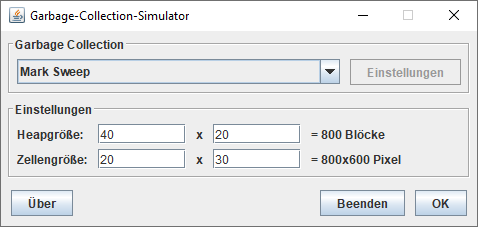
\includegraphics[scale=0.5]{img/gui/selection.png}
	\caption[Auswahlfenster des Simulators]{Auswahlfenster des Simulators.}
	\label{fig:app-start}
\end{figure}

Sobald die Auswahl bestätigt wurde, beginnt der Simulationsmodus (siehe Abbildung~\ref{fig:app-simulation}).
Mithilfe der Eingabekomponenten im oberen Bereich des Kontrollfensters können nun neue Objekte zum Heap hinzugefügt werden.
Die beiden oberen Textfelder \textit{untere Grenze} und \textit{obere Grenze} geben dabei die Größenordnung an, in der sich neu erzeugte Objekte befinden.
Das Textfeld \textit{Verzweigungsgrad} gibt die Wahrscheinlichkeit an, mit der jedes bereits existierende Objekt eine Referenz auf ein neu erstelltes Objekt erhält, während \textit{Anteil Basisobjekte} bestimmt, mit welcher Wahrscheinlichkeit ein erzeugtes Objekt ein Basisobjekt ist.
Die Schaltfläche \textit{Objekt erstellen} erzeugt ein einzelnes Objekt mit den spezifizierten Eigenschaften, während ein Klick auf \textit{Heap füllen} solange Objekte erzeugt, bis ein Allokationsversuch fehlschlägt.
Mittels der Schaltfläche \textit{Heap leeren} kann der Heap zurückgesetzt werden.
Dies ist etwa notwendig, wenn ein Kollektionszyklus unterbrochen wird und sich Objekte mit verschiedenen Markierungen im Heap befinden.
Die Schaltfläche \textit{Heap ausblenden} verbirgt die grafische Ausgabe des Heaps bzw. blendet sie wieder ein.
Im unteren Bereich des Kontrollfensters lässt sich mit dem \textit{Verwaisungsgrad} die Wahrscheinlichkeit einstellen, mit der eine Referenz entfernt wird (siehe auch Abschnitt~\ref{sub:controller}).
Im Textfeld \textit{Animationsgeschwindigkeit} kann der zeitliche Abstand zweier Animationsschritte festgelegt werden (siehe auch Abschnitt~\ref{sec:gui}).
Ein Klick auf \textit{GC ausführen} löst den Garbage-Collection-Algorithmus aus.
Unentdeckte Objekte werden dabei zunächst hellblau dargestellt und bei Entdeckung gelb markiert.
Nach erfolgter Abarbeitung werden sie grün gefärbt.

\begin{figure}[h]
	\centering
	\begin{subfigure}[t]{0.6\textwidth}
		\centering
		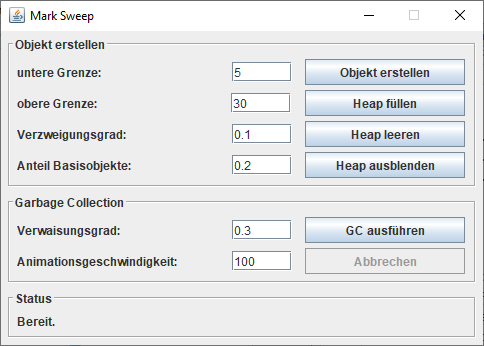
\includegraphics[scale=0.5]{img/gui/simulation-control.png}
		\caption{Kontrollfenster}
	\end{subfigure}~\hspace{0.25cm}~
	\begin{subfigure}[t]{0.35\textwidth}
		\centering
		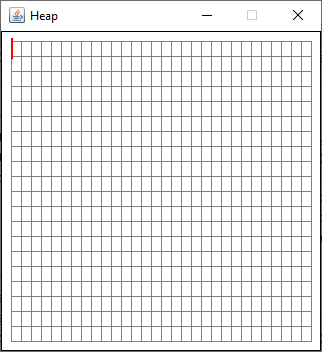
\includegraphics[scale=0.5]{img/gui/simulation-canvas.png}
		\caption{Darstellung des Heaps}
	\end{subfigure}
	\caption[Simulationsmodus]{Simulationsmodus.}
	\label{fig:app-simulation}
\end{figure}

Durch wiederholte Ausführung von Füll- und Kollektionsphasen kann der langfristige Einsatz eines Algorithmus simuliert werden, wobei interessante Eigenschaften beobachtet werden können.
Eine Anpassung der einstellbaren Parameter sorgt dabei für eine Simulation mannigfaltiger Szenarien (siehe Abbildung~\ref{fig:simulation}).
Eine Verwendung unterschiedlich großer Objekte lässt etwa beim Mark-Sweep-Algorithmus die zunehmende Fragmentierung des ungenutzten Speichers erkennen, die Allokationsversuche fehlschlagen lässt.
Dieses Phänomen tritt jedoch nicht auf, wenn die Objektgröße konstant ist.
Beim Lisp-2-Algorithmus ist wiederum zu sehen, dass bei geringem Verwaisungsgrad (bzw. hohem Verzweigungsgrad) die Ausbeute des Kollektors eher gering ist, aber bedingt durch die Kompaktierungsphase dennoch viele Objekte verschoben werden, was sehr zeitaufwendig sein kann.
Eine ähnliche Kausalität kann ebenfalls beim Halbraumverfahren beobachtet werden, wobei hier zusätzlich die Halbierung des Speicherplatzes ins Auge springt.
Objekte, die bei diesem Algorithmus bereits in den anderen Halbraum kopiert wurden, werden hier zusätzlich dunkelblau dargestellt.

\begin{figure}[p]
	\centering
	\begin{subfigure}{\textwidth}
		\centering
		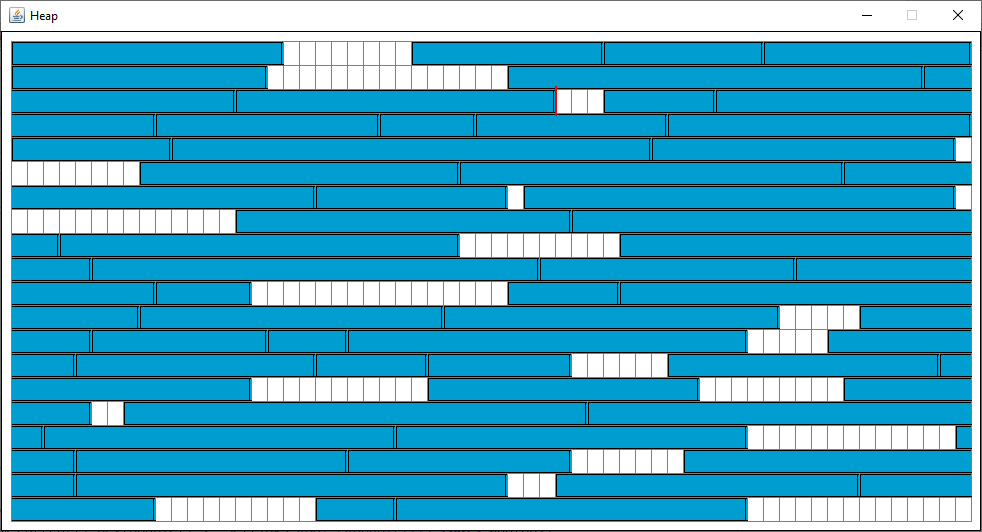
\includegraphics[scale=0.3]{img/gui/marksweep-simulation.png}
		\caption{Nach mehreren Kollektionzyklen lässt sich beim Mark-Sweep-Algorithmus deutlich eine langfristige Fragmentierung des Heaps erkennen.}
	\end{subfigure}\\[0.7cm]
	\begin{subfigure}{\textwidth}
		\centering
		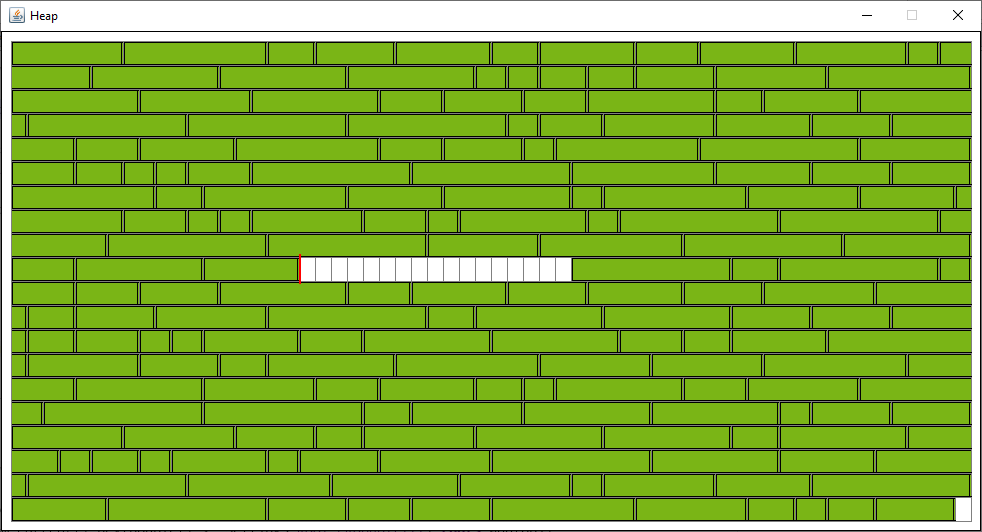
\includegraphics[scale=0.3]{img/gui/lisp2-simulation.png}
		\caption{Bei geringem Verwaisungsgrad ist zu sehen, dass die Kompaktierungsphase des Lisp-2-Algorithmus sehr zeitaufwendig ist, obwohl die Ausbeute eher gering ist.}
	\end{subfigure}\\[0.7cm]
	\begin{subfigure}{\textwidth}
		\centering
		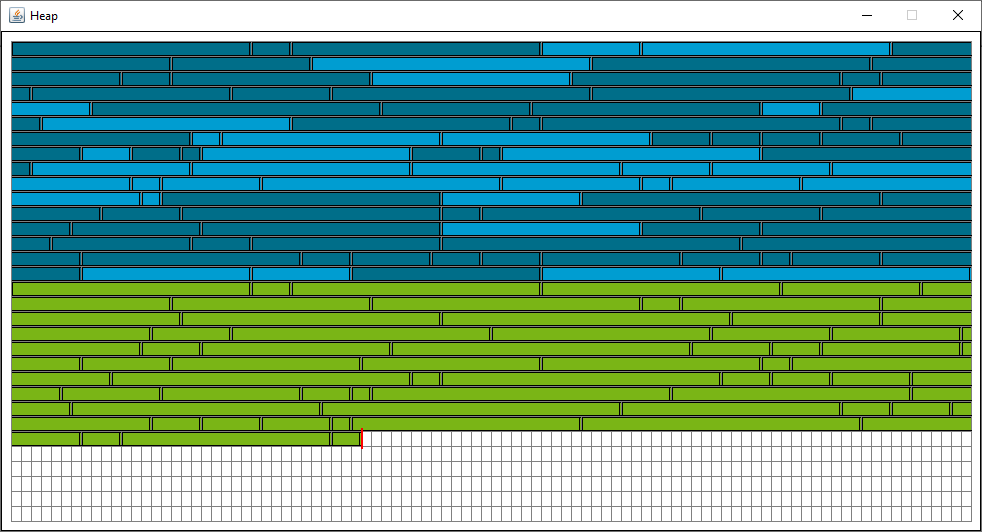
\includegraphics[scale=0.3]{img/gui/semispace-simulation.png}
		\caption{Beim Halbraumverfahren ist die Aufteilung des Heaps in zwei Hälften deutlich zu sehen.}
	\end{subfigure}
	\caption[Simulation der verschiedenen Algorithmen]{Simulation der verschiedenen Algorithmen.}
	\label{fig:simulation}
\end{figure}

\section{Erweiterungsmöglichkeiten}
\label{sec:extension}

\todo[inline]{Erweiterungen: Implementation zusätzlicher Algorithmen, zusätzliche Allokatoren, Grafische Ausgabe mit Graph, um Verwaisung direkter beeinflussen und Referenzmanipulationen und -anpassungen sehen zu können, Stepper mit Swing-Timern}